\section{电荷和电场}
	\subsection{库伦定律}
		真空中静止点电荷Q对另一个静止点电荷Q`的作用力$\boldsymbol{F}$为
			\begin{equation}
			\boldsymbol{F}=\frac{Q Q^{\prime}}{4 \pi \varepsilon_{0} r^{3}} \boldsymbol{r}
			\end{equation}
		其中$\varepsilon_{0}$为真空介电常量。

		现代观点认为两电荷之间的作用力是通过场传递的,由上式可知电荷受到的作用力与电荷量Q成正比,我们定义电场强度$\boldsymbol{E}(x)$来表述电荷之间的作用力
		\begin{equation}
		\boldsymbol{F}=\boldsymbol{Q}^{\prime} \boldsymbol{E}
		\end{equation}
		结合两式可以直接表达出电场强度
		\begin{equation}
			\boldsymbol{E}=\frac{Q \boldsymbol{r}}{4 \pi \varepsilon_{0} r^{3}}
		\end{equation}

		在实际情况中,由于电场具有叠加性,由物体的电荷密度球积分可以得到一个几何物体周围的电场强度分布
		\begin{equation}
		\boldsymbol{E}(x)=\int_{V} \frac{\rho\left(\boldsymbol{x}^{\prime}\right) \boldsymbol{r}}{4 \pi \varepsilon_{0} r^{3}} \mathrm{~d} V^{\prime}
		\end{equation}
	\subsection{高斯定理和电场散度}
		在研究电荷和电场的关系时,我们知道电荷Q发出的电场强度的通量总是正比于Q,与附近其他电荷的存在无关,我们以点电荷周围的闭合曲面S的电场强度E的通量,由高斯定理得
		\begin{equation}
			\oint_{S} \boldsymbol{E} \cdot \mathrm{d} \boldsymbol{S}= \frac{Q}{\varepsilon_0}
		\end{equation}

		将面元投影得到闭合曲面的通量
		\begin{equation}
			\oint_{S} \boldsymbol{E} \cdot \mathrm{d} S=\frac{Q}{4 \pi \varepsilon_{0}} \oint \mathrm{d} \Omega=\frac{Q}{\varepsilon_{0}}
		\end{equation}
		其中$d \Omega$为立体角元。相应的,对于已知的空间电荷分布,对相应的电荷求积分即可得到
		\begin{equation}
			\oint_{s} E \cdot \mathrm{d} S=\frac{1}{\varepsilon_{0}} \int_{V} \rho \mathrm{d} V
		\label{fig.电场通量积分式}
		\end{equation}

		当体积V不断缩小的时候,电场的通量可以改写为散度的形式,有
		\begin{equation}
			\boxed{\boldsymbol{\nabla} \cdot \boldsymbol{E}=\frac{\rho}{\boldsymbol{\varepsilon}_{0}}}
		\end{equation}
		它是电场的一个基本微分方程,反映电场作用的局域性质:\textbf{空间某点领域上场的散度只和点上的电荷密度有关,而和其他地点的电荷分布无关}。特别的,在一般的运动电荷的前提下,远处的场不能用库伦定律表出。
	\subsection{静电场的旋度}
		旋度所反映的是场的环流性质,下面我们用库伦定律来证明电场没有旋度。在电场空间的某个环路中有下面的关系
		\begin{equation}
			\oint_{L} \boldsymbol{E} \cdot \mathrm{d} \boldsymbol{l}=\frac{Q}{4 \pi \varepsilon_{0}} \oint_{L} \frac{\mathrm{d} r}{r^{2}}=-\frac{Q}{4 \pi \varepsilon_{0}} \oint_{L} \mathrm{~d}\left(\frac{1}{r}\right)
		\end{equation}
		\begin{figure}[H]
						\centering  % width栏调节相对行宽的大小
						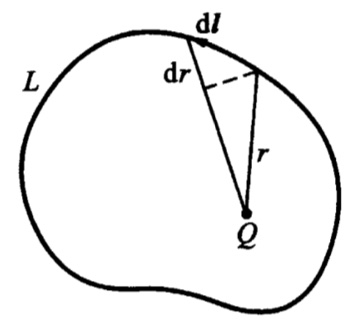
\includegraphics[width=0.2\linewidth]{figs/电场环路.jpg}
						\caption{电场环路} % 图片添加注释
						\label{fig.电场环路}
						\end{figure}

		观察上式得到右边的被积函数是一个全微分,绕L的回路积分值为零。因此得到
			\begin{equation}
				\boxed{\oint_{L} \boldsymbol{E} \cdot \mathrm{d} \boldsymbol{l}=0}
			\end{equation}

		将回路不断缩小,得到静电场的旋度表达
			\begin{equation}
				\boldsymbol{\nabla} \times \boldsymbol{E}=0
			\end{equation}

		电荷是电场的源,电场线从正电荷发出而终止于负电荷,在自由空间中电场线连续通过;在静电情形下电场没有旋涡状结构。
\section{电流和磁场}
		在介绍磁场性质之前,先给出两个电流分布的基本规律。
		\subsection{电荷守恒定律}
			一个系统的总电荷严格保持不变。以电流和电荷的关系用连续性方程表示为
				\begin{equation}
					\oint_{S} \boldsymbol{J} \cdot \mathrm{d} \boldsymbol{S}=\int_V \boldsymbol{\nabla} \cdot \boldsymbol{J} \mathrm{d} V=-\int_{V} \frac{\partial \rho}{\partial t} \mathrm{~d} V
				\end{equation}
			化简得到微分方程
			\begin{equation}
				\boldsymbol{\nabla} \cdot \boldsymbol{J}+\frac{\partial \rho}{\partial t}=0
			\end{equation}
			上式被称为\textbf{电流连续性方程}。特别的,当研究的对象是恒定电流时,物理量不随时间变化,此时$\partial \rho/\partial t=0$,所以在恒定电流情况下
			\begin{equation}
			\boldsymbol{\nabla} \cdot \boldsymbol{J}=0
			\end{equation}
			这一点也可以印证恒定电流的分布是无源的,流线必为闭合曲线。
		\subsection{毕奥-萨伐尔定律}
			该定律描述了两个电流之间的作用力,一个电流元在磁场中受到的力可以表示为
			\begin{equation}
			d \boldsymbol{F}=Id \boldsymbol{l}\times \boldsymbol{B}
			\end{equation}
			给出电流密度之后表示场点上的磁感应强度为
			\begin{equation}
				\boldsymbol{B}(\boldsymbol{x})=\frac{\mu_{0}}{4 \pi} \int_{V} \frac{\boldsymbol{J}\left(\boldsymbol{x}^{\prime}\right) \times \boldsymbol{r}}{r^{3}} \mathrm{~d} V^{\prime}
			\end{equation}
			当电流集中在细导线上,改写定律为
			\begin{equation}
				\boldsymbol{B}(\boldsymbol{x})=\frac{\mu_{0}}{4 \pi} \oint_{L} \frac{I \mathrm{~d} \boldsymbol{l} \times \boldsymbol{r}}{r^{3}}
			\end{equation}
	\subsection{磁场的环量和旋度}
		磁场沿闭合曲线的环量与通过闭合曲线所围曲面的电流I成正比
		\begin{equation}
		\oint_L \boldsymbol{B} \cdot d \boldsymbol{l}=\mu_0 I
		\label{fig.安培环路定律}
		\end{equation}
		上式称为安培环路定律,可以通过毕奥-萨伐尔定律证明,在此不多赘述。

		求得微分形式
		\begin{equation}
			\boldsymbol{\nabla} \times \boldsymbol{B}=\mu_{0} \boldsymbol{J}
		\end{equation}
	\subsection{磁场的散度}
		磁感应强度是无源场,对任何闭合曲面的总通量为零
		\begin{equation}
			\oint_{s} \boldsymbol{B} \cdot \mathrm{d} \boldsymbol{S}=0
		\end{equation}
		微分形式
		\begin{equation}
			\boldsymbol{\nabla} \cdot \boldsymbol{B}=0
		\end{equation}
	\subsection{磁场旋度和散度公式的证明}
\section{麦克斯韦方程组}
	在之前的章节里我们已经讨论了静电磁场的散度和旋度,下面我们考虑变化的电磁场的关系,主要是考虑新增的两个物理量之间的联系
	\begin{enumerate}
	\item 变化的磁场激发电场
	\item 变化的电场激发磁场
	\end{enumerate}

	\subsection{电磁感应定律}
		我们引入线圈L上的感应电动势,已知它和磁通量的变化率成正比。对于闭合线圈而言,感应电动势的存在表面线圈中存在电场,且感应电动势是电场强度沿闭合回路的线积分,综合上述得到
		\begin{equation}
			\oint_{L} \boldsymbol{E} \cdot d \boldsymbol{l}=\mathscr{E}= -\frac{d}{d t} \int_{S} \boldsymbol{B} \cdot d\boldsymbol{S}
		\end{equation}
		微分形式
		\begin{equation}
			\boldsymbol{\nabla} \times \boldsymbol{E}=-\frac{\partial \boldsymbol{B}}{\partial t}
		\end{equation}

		感应电场是有旋场。
	\subsection{位移电流}
		在上一节我们指出恒定电流是闭合的,在交变的情况下,电流分布不再是闭合的——可以用带电容器的电路为例,实际上该处的电流是中断的。

		恒定电流满足安培环路定律\ref{fig.安培环路定律},对式子两边取散度,由于$\nabla \cdot \nabla \times \boldsymbol{B} \equiv 0$,上式只有当$\nabla \cdot \boldsymbol{J}=0$的时候成立,而恒定电流下无磁场产生,因此两者相互矛盾。

		我们假设存在一个位移电流$\boldsymbol{J}_D$,使得它和电流$\boldsymbol{J}$合起来构成闭合的电流,满足
		\begin{equation}
		\nabla \cdot\left(\boldsymbol{J}+\boldsymbol{J}_{\mathrm{D}}\right)=0
		\label{eq.位移电流定义式}
		\end{equation}
		这样可以解决前文的矛盾,现在只需要表示出位移电流,联立
		\begin{equation}
		\begin{gathered}
			\nabla \cdot \boldsymbol{J}+\frac{\partial \rho}{\partial t}=0 \\
			\nabla \cdot \boldsymbol{E}=\frac{\rho}{\varepsilon_{0}}
		\end{gathered}
		\end{equation}
		得到$\boldsymbol{J}_D$的一个可能的表达式\footnote{实际上由式\ref{eq.位移电流定义式}可以得到多个可能的解,只是该解是最简单的求解}
		\begin{equation}
			\boldsymbol{J}_{\mathbf{D}}=\varepsilon_{0} \frac{\partial \boldsymbol{E}}{\partial t}
		\end{equation}

		\par \qquad

		综上所述,得到MaxWell方程组
		\begin{equation}
			\boxed{\begin{gathered}
		\boldsymbol{\nabla} \times \boldsymbol{E}=-\frac{\partial \boldsymbol{B}}{\partial t} \\
		\boldsymbol{\nabla} \times \boldsymbol{B}=\mu_{0} \boldsymbol{J}+\mu_{0} \varepsilon_{0} \frac{\partial \boldsymbol{E}}{\partial t} \\
		\boldsymbol{\nabla} \cdot \boldsymbol{E}=\frac{\rho}{\varepsilon_{0}} \\
		\boldsymbol{\nabla} \cdot \boldsymbol{B}=0
		\end{gathered}}
		\end{equation}

	\subsection{洛伦兹力公式}
		场对电荷体系的作用分别表述为电场和磁场之间的作用,通过库仑定律和安培定律体现,分别是
			\begin{equation}
				\begin{aligned}
				\vec{F}&=Q \vec{E} \\
				d \vec{F}&=I d \vec{l} \times \vec{B}=\vec{J} \times \vec{B} d V
				\end{aligned}
			\end{equation}

		两者相加并写作力密度的形式
			\begin{equation}
			\vec{f}=\rho \vec{E}+\vec{J} \times \vec{B}
			\end{equation}

		对于单个点电荷,很容易得到关系$\vec{J}=\rho \vec{v}$

		化简得
			\begin{equation}
				\vec{F}=q \vec{E}+q \vec{v} \times \vec{B}
			\end{equation}

\section{介质的电磁性质}
	介质是一个带电粒子系统,在介质被极化的时候,由正点中心和负电中心是否重合分为两类:重合的介质在
		\begin{figure}[H]
			\centering  % width栏调节相对行宽的大小
			
\includegraphics[width=0.8\linewidth]{figs/电磁介质.jpg}
			\caption{电磁介质} % 图片添加注释
			\label{fig.电磁介质}
		\end{figure}

	\subsection{介质的极化}
		\begin{wrapfigure}{r}{4cm}%靠文字内容的右侧
      		\centering
      		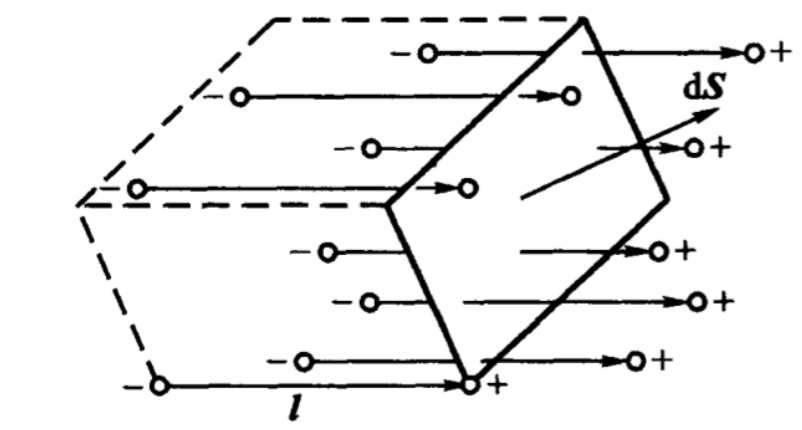
\includegraphics[width=0.28\textwidth]{figs/介质极化示意图.jpeg}
      		\caption{介质的极化}
      		\label{fig.介质的极化}
      		\end{wrapfigure}
      		在外场的作用下,介质中的正负电子对会一致取向排列,形成有图的排列。如果正电荷在外,那么介质中便有等量的负电荷来维持介质的整体电中性。\textbf{这种由于极化而出现的电荷分布称为束缚电荷},以$\rho_p$表示束缚电荷密度,有关系
		\begin{equation}
			\int_{V} \rho_{\mathrm{P}} \mathrm{d} V=-\oint_{S} \boldsymbol{P} \cdot \mathrm{d} S
		\end{equation}
		对于体积分的表示,则可以表达为
			\begin{equation}
			\rho_p=- \nabla \cdot \mathbf{P}
			\end{equation}
		
		非均匀介质极化后整个介质内部都有束缚电荷出现,而在均匀介质内,束缚电荷字出现在自由电荷附近和介质界面处。我们需要特别说明的是介质分界面上束缚电荷的表示,由上图\ref{fig.介质的极化}可以得知——在两个介质的分界面,介质1和介质2分别都有本介质极化后的剩余电荷和另一个介质“漂移”过来的电荷,在分界面薄层出现的净余电荷就可以表示为$-\left(\boldsymbol{P}_{2}-\boldsymbol{P}_{1}\right) \cdot \mathrm{d} \boldsymbol{S}$,其中有束缚电荷面密度$\sigma_p$,则进一步表示为
		\begin{equation}
			\boldsymbol{\sigma}_{\mathrm{P}} \mathrm{d} S=-\left(\boldsymbol{P}_{2}-\boldsymbol{P}_{1}\right) \cdot \mathrm{d} \boldsymbol{S}
		\end{equation}
		\begin{equation}
			\sigma_{\mathrm{P}}=-\boldsymbol{e}_{\mathbf{n}} \cdot\left(\boldsymbol{P}_{2}-\boldsymbol{P}_{1}\right)
		\end{equation}
		介质内的电现象包括两个方面.一方面电场使介质极化而产生束缚电荷分布,另一方面这些束缚电荷又反过来激发电场,两者是互相制约的。\textbf{介质对宏观电场的作用就是通过束缚电荷激发电场。}

		所以整体仍然满足Maxwell方程
			\begin{equation}
				\varepsilon_{0} \nabla \cdot \boldsymbol{E}=\rho_{\mathrm{f}}+\rho_{\mathrm{p}}
				\label{eq.1.32}
			\end{equation}
		由于束缚电荷不易测量,更容易得到的是自由电荷,我们引入辅助量电位移矢量$\mathbf{D}$,定义为
		\begin{equation}
			\boldsymbol{D}=\varepsilon_{0} \boldsymbol{E}+\boldsymbol{P}
		\end{equation}
		可以看出,$\mathbf{D}$并不能代表介质中的场强,仅仅有着辅助的作用
		代入上式得到关系
		\begin{equation}
			\nabla \cdot  \boldsymbol{D}=\rho_{f}
		\end{equation}

		极化强度矢量毫无疑问与外电场强度呈某种比例关系,对于一般的各向同性线性介质,极化强度和电场强度有着线性关系
		\begin{equation}
			\boldsymbol{P}=\chi_{\mathrm{e}} \varepsilon_{0} \boldsymbol{E}
		\end{equation}
		联立上式很容易得到关系
		\begin{equation}
			\boldsymbol{D}=\varepsilon \bar{E}
		\end{equation}
		\begin{equation}
			\varepsilon=\varepsilon_{\mathrm{r}} \varepsilon_{0}, \quad \varepsilon_{\mathrm{r}}=1+\chi_{\mathrm{e}}
		\end{equation}
		$\varepsilon$ 称为介质的电容率, $\varepsilon_{\mathrm{r}}$为相对电容率。

		我们需要明确的是
		\begin{enumerate}
		\item 电场E是电场的基本物理量,代表介质中的总宏观电场强度
		\item 电位移矢量仅仅只是一个辅助量,用于方便的建立与介质自由电荷之间的关系
		\end{enumerate}

		
	\subsection{介质的磁化}
		\begin{wrapfigure}{r}{4.5cm}%靠文字内容的右侧
	      \centering
	      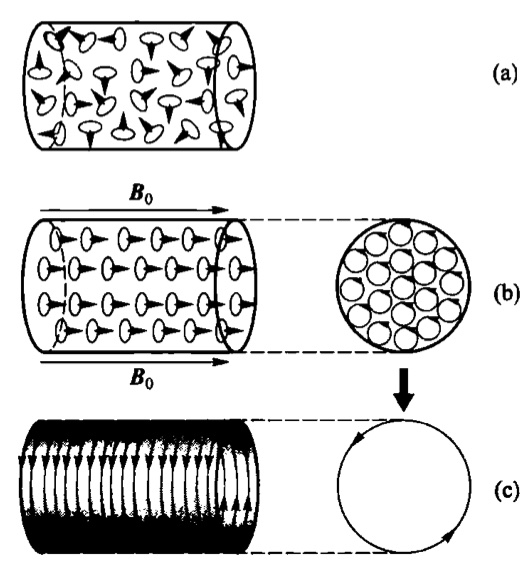
\includegraphics[width=0.2\textwidth]{figs/分子电流磁化.jpg}
	      \caption{分子电流磁化}
	      \end{wrapfigure}
		目前介质磁化的理论解释有两种——分子电流观点和磁荷观点,我们在这里以分子电流为例。

		为使得介绍的流程更加明晰,我们先直接写出麦克斯韦方程组在介质中的满足的方程
		\begin{equation}
		\label{eq.4.16}
			\frac{1}{\mu_{0}} \boldsymbol{\nabla} \times \boldsymbol{B}=\boldsymbol{J}_{\mathrm{f}}+\boldsymbol{J}_{\mathrm{M}}+\boldsymbol{J}_{\mathrm{P}}+\varepsilon_{0} \frac{\partial \boldsymbol{E}}{\partial t}
		\end{equation}

		其中$\boldsymbol{J}_{\mathrm{f}}$为介质中的自由电流密度,$\boldsymbol{J}_{\mathrm{M}}$为介质中的磁化电流密度,$\boldsymbol{J}_{\mathrm{P}}$为介质中的极化电流密度,后两者一并称为\textbf{诱导电流密度}。下面介绍它们的形成机理。

		对于磁化电流密度。为描述磁介质的磁化状态,引入磁化强度矢量,定义为单位体积内分子磁矩的矢量和,我们把宏观体积元内的分子看作电流环,那么只要刚刚与面边缘相交的环对介质磁化有着共贡献,那么可以得到关系
		\begin{equation}
			\oint_{L} M \cdot \mathrm{d} l=\sum_{(L \text { 内) }} I^{\prime}
		\end{equation}
		相应的微分形式为
		\begin{equation}
			J_{M}=\nabla \times M
		\end{equation}

		而对于极化电流密度而言,是电场变化导致的介质极化强度变化而产生的电流,满足
		\begin{equation}
			\frac{\partial \boldsymbol{P}}{\partial t}=\frac{\sum_{i} e_{i} \boldsymbol{v}_{i}}{\Delta V}=\boldsymbol{J}_{\mathrm{P}}
		\end{equation}

		和介质的电场规律一样,自由电流的分布可以直接通过实验测得,我们希望引入一个物理量使得它仅由介质性质和自由电流的分布决定,由上式变化得
		\begin{equation}
			\boldsymbol{\nabla} \times\left(\frac{\boldsymbol{B}}{\mu_{0}}-\boldsymbol{M}\right)=\boldsymbol{J}_{\mathrm{f}}+\frac{\partial \boldsymbol{D}}{\partial t}
		\end{equation}

		引入磁场强度$\mathbf{H}$,定义为
		\begin{equation}
			\mathbf{H}=\frac{\boldsymbol{B}}{\mu_{0}}-\mathbf{M}
		\end{equation}

		这样就有关系
		\begin{equation}
		\label{eq.4.19}
			\boldsymbol{\nabla} \times \mathbf{H}=\boldsymbol{J}_{\mathrm{f}}+\frac{\partial \mathbf{D}}{\partial t}
		\end{equation}
		从式\ref{eq.4.16}和式\ref{eq.4.19}可以看出,磁感应强度B描述了介质内整体的宏观磁场,而H仅仅只是一个辅助物理量,为能完备的描述H和B之间的关系,我们还需要介质的磁化率$\chi_M$。对于各向同性非铁磁物质而言,上式的几个物理量之间有着线性关系\footnote{为什么讨论磁介质的时候要考虑极化带来的影响,而讨论极化的时候没有与磁化相关的项}
		\begin{equation}
			\mathbf{M}=\chi_{\mathrm{M}} \mathbf{H}
		\end{equation}
		\begin{equation}
			B=\mu \mathbf{H}
		\end{equation}
		\begin{equation}
			\mu=\mu_{\mathrm{r}} \mu_{0}, \quad \mu_{\mathrm{r}}=1+\chi_{\mathrm{M}}
		\end{equation}
	\subsection{介质中的Maxwell方程组}
		\begin{equation}
		\boxed{
			\begin{aligned}
			&\nabla \times \boldsymbol{E}=-\frac{\partial \boldsymbol{B}}{\partial t} \\
			&\nabla \times \boldsymbol{H}=\boldsymbol{J}+\frac{\partial \mathbf{D}}{\partial t} \\
			&\nabla \cdot \boldsymbol{D}=\rho \\
			&\nabla \cdot \boldsymbol{B}=0
			\end{aligned}}
		\end{equation}
		式中出现的$\rho$等符号都是直接代指自由电荷和自由电流的分布。

		上述方程组想要求解还需要下面的一些关系
		\begin{equation}
			\begin{aligned}
			&\boldsymbol{D}=\varepsilon \bar{E} \\
			&\boldsymbol{B}=\mu \boldsymbol{H} \\
			&\boldsymbol{J}=\sigma \bar{E}
			\end{aligned}
		\end{equation}
		注意,这只在部分的各向同性介质中成立,对于更复杂的异性介质,可能需要张量式来描述
		\vspace*{2em}

		在介质中电场磁场相应的对应关系为
		
		\begin{figure}[H]
						\centering  % width栏调节相对行宽的大小
						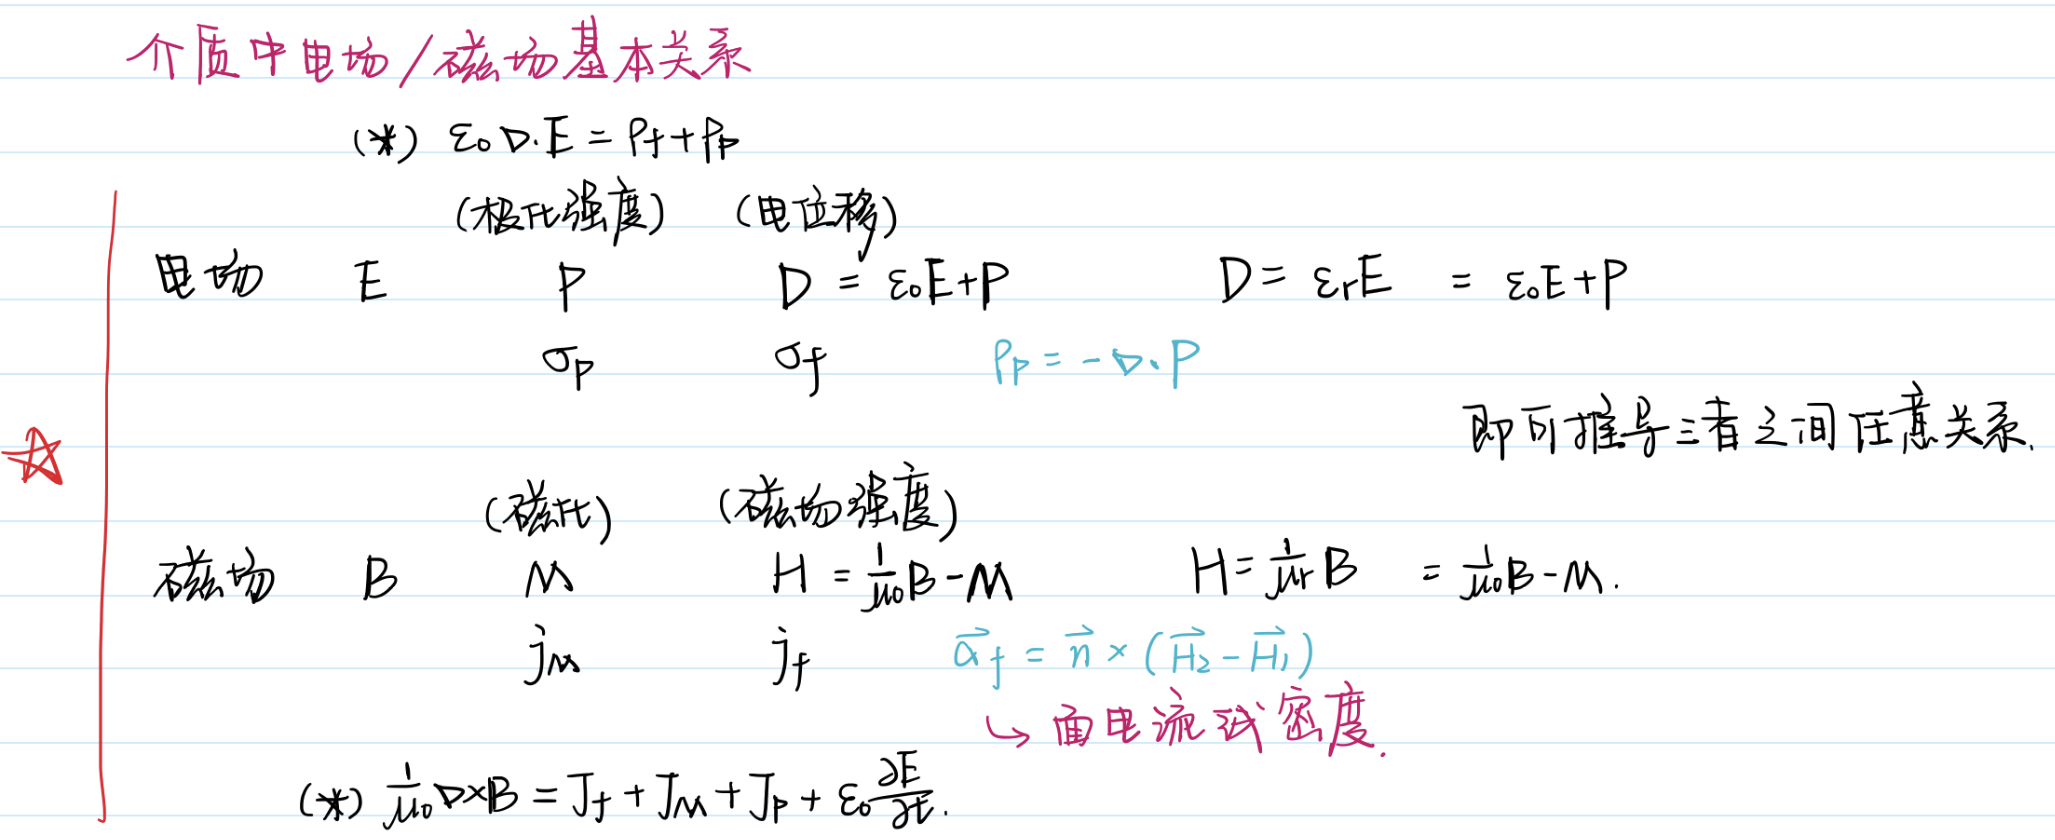
\includegraphics[width=0.9\linewidth]{figs/介质中电场磁场对应关系.jpeg}
						\caption{介质中电场磁场对应关系} % 图片添加注释
						\label{fig.介质中电场磁场对应关系}
						\end{figure}
	\section{电磁场边值关系}
		我们在本节的开始直接给出积分形式的介质内麦克斯韦方程组,根据下式我们可以很直观的推导出电磁场的边值关系
			\begin{equation}
				\label{eq.1_53}
				\begin{aligned}
				&\oint_{L} \boldsymbol{E} \cdot \mathrm{d} \boldsymbol{l}=-\frac{\mathrm{d}}{\mathrm{d} t} \int_{S} \boldsymbol{B} \cdot \mathrm{d} \boldsymbol{S} \\
				&\oint_{L} \boldsymbol{H} \cdot \mathrm{d} \boldsymbol{l}=I_{\mathrm{f}}+\frac{\mathrm{d}}{\mathrm{d} t} \int_{S} \boldsymbol{D} \cdot \mathrm{d} \boldsymbol{S} \\
				&\oint_{S} \boldsymbol{D} \cdot \mathrm{d} \boldsymbol{S}=\boldsymbol{Q}_{\mathrm{f}} \\
				&\oint_{S} \boldsymbol{B} \cdot \mathrm{d} \boldsymbol{S}=0
				\end{aligned}
				\end{equation}
		\subsection{法向分量的关系}
			总电场的Maxwell方程组有
				\begin{equation}
					\varepsilon_{0} \oint_{S} \boldsymbol{E} \cdot \mathrm{d} \boldsymbol{S}=Q_{\mathrm{f}}+Q_{\mathrm{P}}
				\end{equation}
			如果在边界面上取一个厚度几乎为零的圆柱体,那么上式的面积分就等价于$\left(E_{2 \mathrm{n}}-E_{1 \mathrm{n}}\right) \Delta S$,对于上式而言,及方程左边化为面密度的物理量,即
				\begin{equation}
					\varepsilon_{0}\left(E_{2 \mathrm{n}}-E_{1 \mathrm{n}}\right)=\sigma_{\mathrm{f}}+\sigma_{\mathrm{P}}
				\end{equation}
			本式在前文讨论介质极化的时候已经提到过,见式\ref{eq.1.32}

			同样的,根据介质极化的相关结论,我们可以得到
			\begin{equation}
				P_{2 \mathrm{n}}-P_{1 \mathrm{n}}=-\sigma_{\mathrm{P}}
			\end{equation}
			\begin{equation}
				\boxed{D_{2 \mathrm{n}}-D_{1 \mathrm{n}}=\sigma_{\mathrm{f}}}
			\end{equation}

			可以看出,与介质极化相关的这三个物理量,以及三者在法向上的跃变,分别受不同的电荷面密度影响。

			相应的,对于磁场满足
			\begin{equation}
				\oint_{S} \boldsymbol{B} \cdot \mathrm{d} \boldsymbol{S}=0
			\end{equation}
			同样的利用取薄圆柱体的方法,容易得到
			\begin{equation}
				\boxed{B_{2 \mathrm{n}}=B_{1 \mathrm{n}}}
			\end{equation}
		\subsection{切向分量的关系}
		\begin{wrapfigure}{r}{4.5cm}%靠文字内容的右侧
	      \centering
	      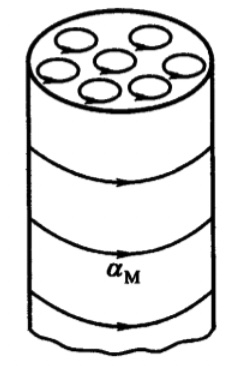
\includegraphics[width=0.12\textwidth]{figs/磁化面电流示意图.jpg}
	      \caption{磁化面电流示意图}
	      \end{wrapfigure}
			先明确面电流分布——及体电流分布在宏观上等效于表面电流分布的一种考虑情况,我们假设面电流线密度为$\alpha$,则垂直流过一段距离的电流表示为
			\begin{equation}
				\Delta I=\alpha \Delta l
			\end{equation}

			根据式\ref{eq.1_53}第二式可以得知求解磁场的边值关系需要的两个物理量——$I_f$和$ \int_{S} \boldsymbol{D} \cdot \mathrm{d} \boldsymbol{S}$。

			我们选取介质表面一个宽度趋近于零的矩形,面电流的方向垂直于平面方向,如图\ref{fig.切向分量边值关系示意图}。
			\begin{figure}[H]
				% centering使图片居中
				\centering  % width栏调节相对行宽的大小
				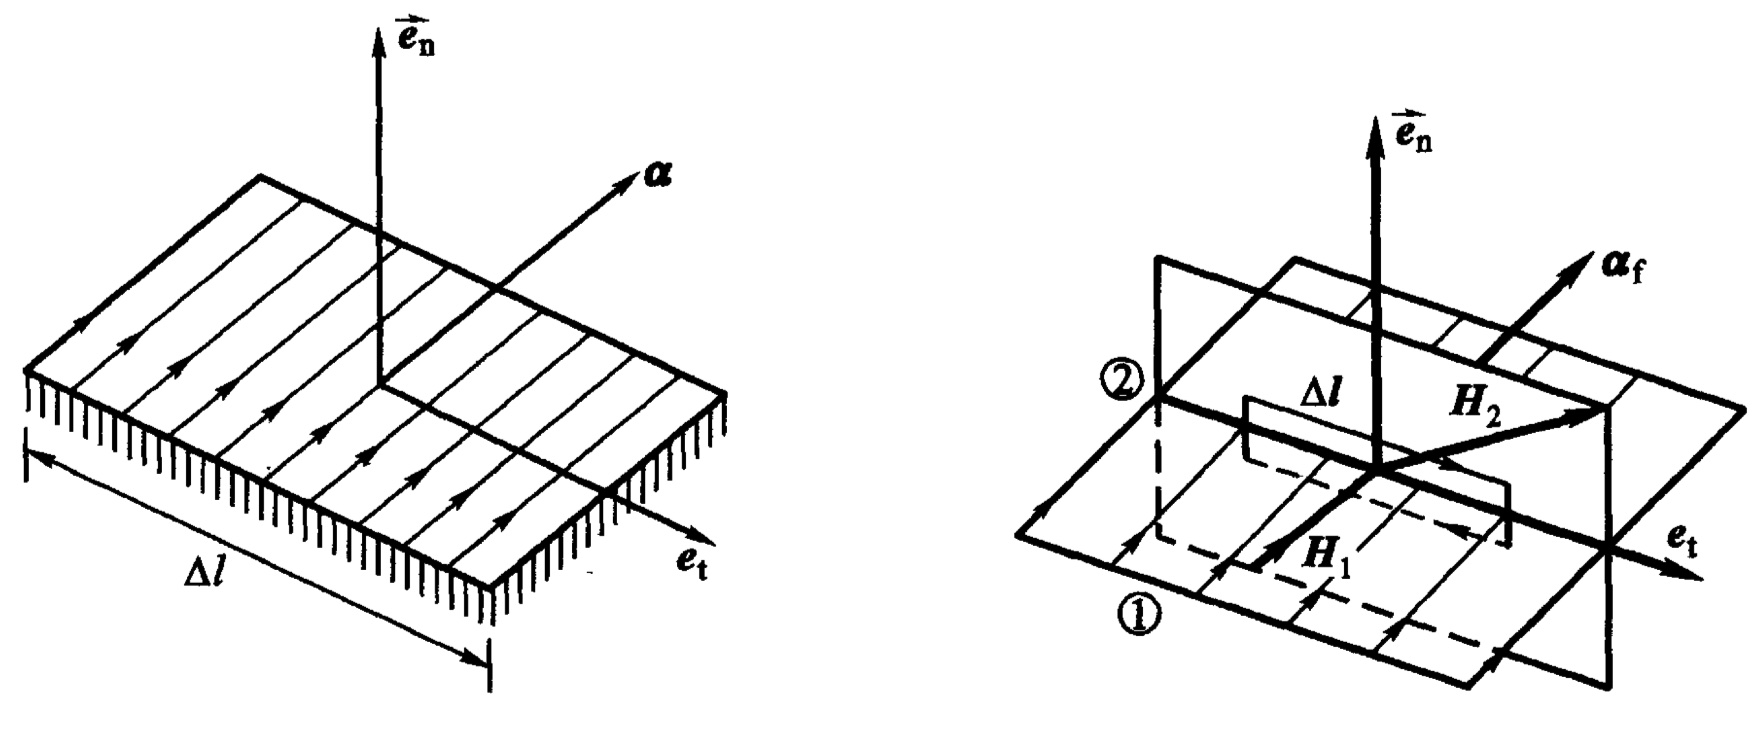
\includegraphics[width=0.7\linewidth]{figs/切向分量边值关系示意图.jpg}
				\caption{切向分量边值关系示意图} % 图片添加注释
				\label{fig.切向分量边值关系示意图}
				\end{figure}
			由于这个回路的面积趋近于零且电位移矢量D有限大,则
			\begin{equation}
			\frac{\mathrm{d}}{\mathrm{d} t} \int_{S} \boldsymbol{D} \cdot \mathrm{d} \boldsymbol{S} \to 0
			\end{equation}
			另一项的推导也非常的明显
			\begin{equation}
				\oint_L \boldsymbol{H} \cdot d \boldsymbol{l} = (H_{2t}-H_{1t}) \Delta l = \alpha_f \Delta l
			\end{equation}
			即
			\begin{equation}
				H_{2 \mathrm{t}}-H_{1 \mathrm{t}}=\alpha_{f}
			\end{equation}

			刚刚给出的分量形式的边值关系,对于一般的矢量
			\begin{equation}
				\boxed{\boldsymbol{e}_{\mathrm{n}} \times\left(\boldsymbol{H}_{2}-\boldsymbol{H}_{1}\right)=\boldsymbol{\alpha}_{f}}
			\end{equation}
			同理,电场的情况就要简单很多
			\begin{equation}
				\boxed{\boldsymbol{e}_{\mathrm{n}} \times (\boldsymbol{E}_2 - \boldsymbol{E}_1) = 0}
			\end{equation}
			
			\vspace*{3em}
			对于自由电荷面密度$\sigma$和自由电流线密度${\boldsymbol{\alpha}_f}$我们能够总结出边值关系为(其中$\boldsymbol{e}_{\mathrm{n}}$是由介质1指向介质2的单位法向量。
			\begin{equation}
				\begin{aligned}
				&\boldsymbol{e}_{\mathrm{n}} \times\left(\boldsymbol{E}_{2}-\boldsymbol{E}_{1}\right)=0 \\
				&\boldsymbol{e}_{\mathrm{n}} \times\left(\boldsymbol{H}_{2}-\boldsymbol{H}_{1}\right)=\boldsymbol{\alpha} \\
				&\boldsymbol{e}_{\mathrm{n}} \cdot\left(\boldsymbol{D}_{2}-\boldsymbol{D}_{1}\right)=\sigma \\
				&\boldsymbol{e}_{\mathrm{n}} \cdot\left(\boldsymbol{B}_{2}-\boldsymbol{B}_{1}\right)=0
				\end{aligned}
				\end{equation}
	\section{电磁场的能量和能流}
		\subsection{场与电荷系统的能量守恒关系}
			由于场的运动能量具有方向性,在不同方向相同距离测量场源发射的强度可能会得到不同的结果,所以对于场的能量的描述,需要两个物理量
				\begin{enumerate}
					\item 场的能量密度$\omega$,它代表场内单位体积的能量,与空间位置和时间有关
					\item 场的能流密度$\boldsymbol{S}$,它代表能量在场内的传播,在数值上等于单位时间垂直流过单位横截面的能量,其方向代表能量传输的方向
				\end{enumerate}
			
			对于空间中某区域V,我们考虑外界流入能量、区域内场和电荷相互作用引起的能量改变、区域内场的总能量的变化这三者之间的关系。首先以$\boldsymbol{f}$	表示场对电荷作用力的密度,$\boldsymbol{v}$表示电荷运动的速度,则场对电荷作用的功率为
			% 本Latex文稿从这里开始不再对临时使用的解释型方程编号
				\begin{equation*}
					\int_V \boldsymbol{f} \cdot \boldsymbol{v} 
				\end{equation*}
			
			同样给出区域内场的能量增加率
				\begin{equation*}
					\frac{d}{dt}\int_V \omega dV
				\end{equation*}
			以上的两个量都可以视作区域内场和电荷体系的“内能”,通过界面S进入区域的能量为
				\begin{equation*}
					-\oint_S \boldsymbol{S} \cdot d \boldsymbol{\sigma}
				\end{equation*}
			
			由能量守恒定律,内部能量变化等于与外界进行的能量交换
				\begin{equation}
					-\oint_S \boldsymbol{S} \cdot d \boldsymbol{\sigma} = \frac{d}{dt}\int_V \omega dV +\int_V \boldsymbol{f} \cdot \boldsymbol{v} 
				\end{equation}
			给出微分形式
				\begin{equation}
					\label{eq.1_68}
					\nabla \cdot \boldsymbol{S}+\frac{\partial \omega}{\partial t}= -\boldsymbol{f} \cdot	\boldsymbol{v}
				\end{equation}
			特别的,如果我们选取的是全空间作为区域,则不存在与外部的能量交换$\nabla \cdot \boldsymbol{S}=0$。这样就代表场对电荷作用的功率等于场自身的能量变化,证明了场和电荷组成的体系能量守恒。

			\subsection{电磁场能量密度和能流密度的表达式}
				由麦克斯韦方程组和洛伦兹力公式进行推导,用洛伦兹力公式表示场对电荷的功率
					\begin{equation}
						\boldsymbol{f} \cdot \boldsymbol{v}=(\rho \boldsymbol{E} + \rho \boldsymbol{v} \times \boldsymbol{B})\cdot \boldsymbol{v} = \rho \boldsymbol{E} \cdot \boldsymbol{v}=\boldsymbol{J} \cdot \boldsymbol{E}
					\end{equation}
				将上式整理为与电磁场场量相关的物理量表示即可
					\begin{equation*}
						\boldsymbol{J} \cdot \boldsymbol{E} = (\nabla \times \boldsymbol{H}-\frac{\partial \boldsymbol{D}}{\partial t})\cdot \boldsymbol{E} = \boldsymbol{E} \cdot (\nabla \times \boldsymbol{H})- \boldsymbol{E} \cdot \frac{\partial \boldsymbol{D}}{\partial t}
					\end{equation*}
				用矢量分析公式得到
					\begin{equation*}
						\begin{aligned}
						\boldsymbol{E} \cdot(\boldsymbol{\nabla} \times \boldsymbol{H}) &=-\nabla \cdot(\boldsymbol{E} \times \boldsymbol{H})+\boldsymbol{H} \cdot(\boldsymbol{\nabla} \times \boldsymbol{E}) \\
						&=-\nabla \cdot(\boldsymbol{E} \times \boldsymbol{H})-\boldsymbol{E} \cdot \frac{\partial \boldsymbol{B}}{\partial t}
						\end{aligned}
					\end{equation*}
				代入上式得到关系
				\begin{equation}
					\boldsymbol{J} \cdot \boldsymbol{E}=-\boldsymbol{\nabla} \cdot(\boldsymbol{E} \times \boldsymbol{H})-\boldsymbol{E} \cdot \frac{\partial \boldsymbol{D}}{\partial t}-\boldsymbol{H} \cdot \frac{\partial \boldsymbol{B}}{\partial t}
				\end{equation}

				对比式\ref{eq.1_68}可以找到能量密度和能流密度。其中能流密度也称为Poynting矢量。
				\begin{equation}
					\label{eq.1_71}
					\boxed{\begin{gathered}
					\boldsymbol{S}=\boldsymbol{E} \times \boldsymbol{H} \\
					\frac{\partial w}{\partial t}=\boldsymbol{E} \cdot \frac{\partial \boldsymbol{D}}{\partial t}+\boldsymbol{H} \cdot \frac{\partial \boldsymbol{B}}{\partial t}
					\end{gathered}}
				\end{equation}

				我们在两种最常见的情况下讨论我们的结果
				\begin{enumerate}[I.]
					\item 真空中电荷分布的情形
							\begin{equation*}
								\boldsymbol{H}=\frac{1}{\mu_0}\boldsymbol{B}, \qquad \boldsymbol{D}=\varepsilon_0 \boldsymbol{E}
							\end{equation*}
						直接代入式\ref{eq.1_68},可以得到
							\begin{eqnarray}
								\begin{gathered}
									\boldsymbol{S} =\frac{1}{\mu_0} \boldsymbol{E} \times \boldsymbol{B} \\
									\omega = \frac{1}{2}(\varepsilon_0 E^2+\frac{1}{\mu_0} B^2)
								\end{gathered}
							\end{eqnarray}
					\item 介质中分布的情形。在介质中,原本场和自由电荷之间的关系增加了一个与介质的关系,这时候磁化能和极化能需要一起归入考虑。一般的,可以写作
						\begin{equation}
							\delta \omega = \boldsymbol{E}\cdot \delta \boldsymbol{D}+ \boldsymbol{H}\cdot \delta \boldsymbol{B}
						\end{equation}

					特别的,在线性介质中我们可以和真空的情况一起考虑
					\begin{equation*}
						\boldsymbol{H}=\frac{1}{\mu}\boldsymbol{B}, \qquad \boldsymbol{D}=\varepsilon \boldsymbol{E}
					\end{equation*}
					代表电导率和磁导率与空间位置无关,这种情况下取微分就等于
					\begin{equation}
						\label{eq.1_74}
						w=\frac{1}{2}(\boldsymbol{E} \cdot \boldsymbol{D}+\boldsymbol{H} \cdot \boldsymbol{B})=\frac{1}{2}\left(\varepsilon E^{2}+\frac{1}{\mu} B^{2} \cdot\right)
					\end{equation}
				\end{enumerate}
